\documentclass[aspectratio=169]{beamer}

\usepackage[utf8]{inputenc}
\usepackage[T2A]{fontenc}
\usepackage[russian]{babel}
\usepackage{amsmath}
\usepackage{graphicx}
\usepackage{booktabs}

\usetheme{default}
\setbeamertemplate{navigation symbols}{}
\setbeamertemplate{footline}[frame number]

\title{Модель связи валютного курса EUR/USD и цены на нефть Brent}
\author{}
\date{10 марта 2026 года}

\begin{document}

\begin{frame}
\titlepage
\end{frame}

\begin{frame}{Постановка задачи}
\begin{itemize}
    \item Цель проекта: проверить, есть ли устойчивая связь между нефтью Brent и курсом EUR/USD.
    \item Практический смысл: можно ли использовать нефть как фактор валютного риска и ребалансировки.
    \item Основной вопрос: одинакова ли эта связь в долгом и коротком горизонтах.
\end{itemize}
\end{frame}

\begin{frame}{Литература}
\begin{itemize}
    \item Benlaria et al. (2020): ARDL на месячных данных, краткосрочная связь между нефтью и EUR/USD.
    \item Fratzscher, Schneider, Van Robays (2014): связь нефти и доллара усилилась с начала 2000-х, возможна смена рыночных режимов.
    \item Dias et al. (2025): в период 2022--2024 влияние нефти на валюты есть, но для EUR/USD оно уже не выглядит простым и постоянным.
\end{itemize}
\end{frame}

\begin{frame}{Данные и модель}
\begin{itemize}
    \item Источник данных: FRED, ряды \texttt{DEXUSEU} и \texttt{DCOILBRENTEU}.
    \item Дневная выборка: 14.01.2000 -- 02.03.2026.
    \item Месячная выборка: январь 1999 -- февраль 2026.
    \item Краткосрочная модель:
    \[
    \Delta e_t=\alpha+\beta_0\Delta o_t+\beta_1\Delta o_{t-1}+\gamma\Delta e_{t-1}+\varepsilon_t.
    \]
    \item Долгосрочная часть: тест Энгла--Грейнджера и ECM.
\end{itemize}
\end{frame}

\begin{frame}{Главный краткосрочный результат}
\begin{itemize}
    \item Полная выборка 2010--2026: коэффициент при текущей доходности нефти $\beta_0 \approx 0.014$, $p \approx 0.006$.
    \item Подвыборка 2010--2021: $\beta_0 \approx 0.016$, $p \approx 0.009$.
    \item Подвыборка 2022--2026: $\beta_0 \approx 0.004$, $p \approx 0.709$.
    \item Вывод: краткосрочная связь есть, но в последние годы она стала заметно слабее.
\end{itemize}
\end{frame}

\begin{frame}{Визуализация связи}
\begin{center}
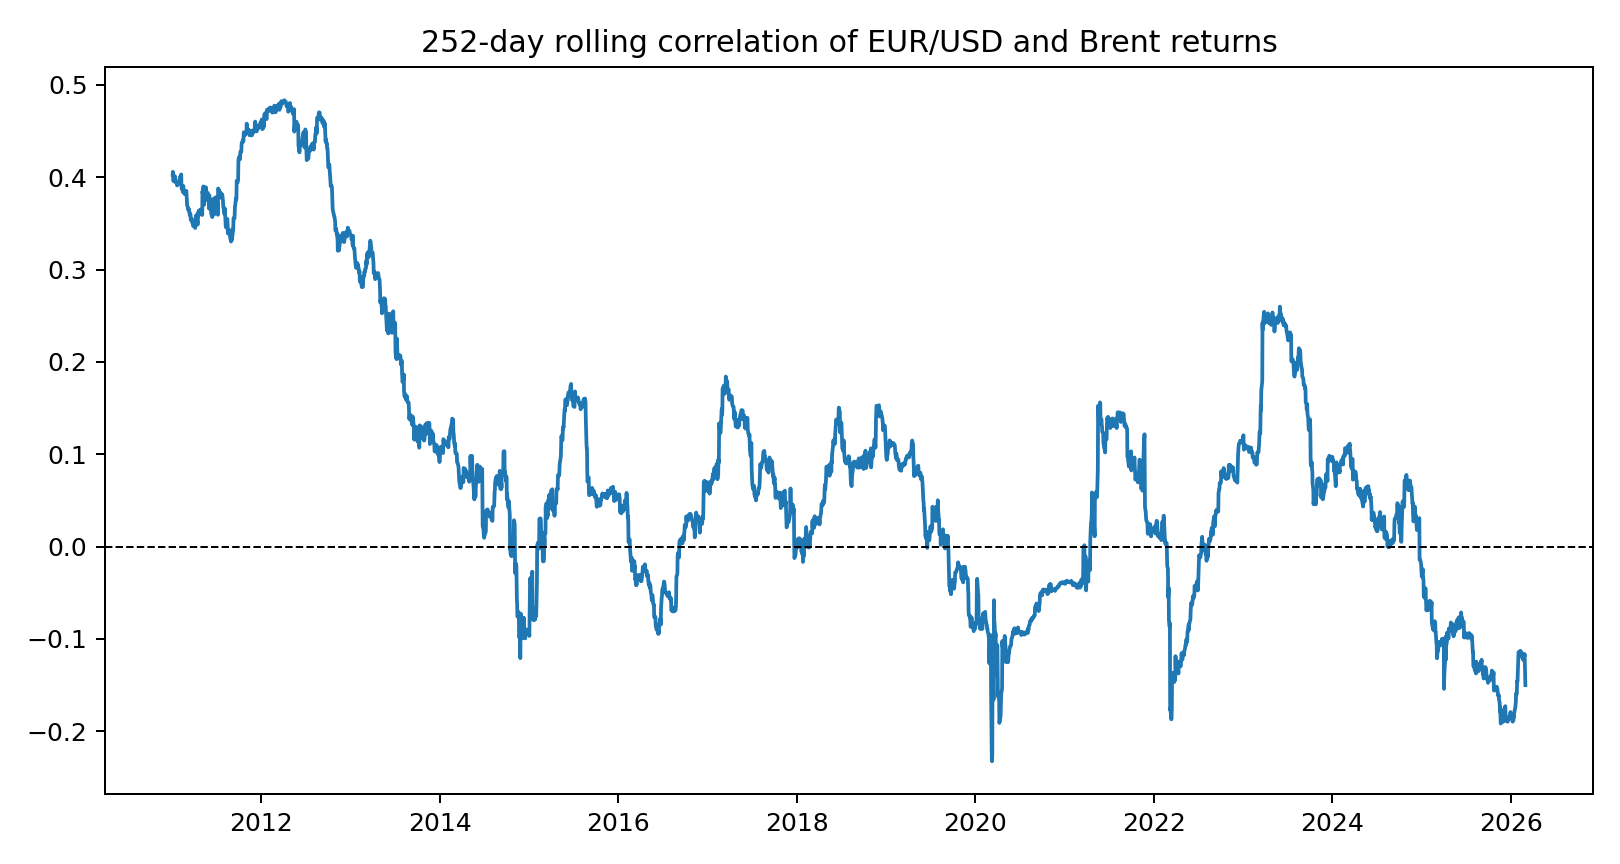
\includegraphics[width=0.82\textwidth]{results/rolling_correlation.png}
\end{center}
\begin{itemize}
    \item Скользящая корреляция заметно меняется по времени.
    \item Следовательно, нефть нельзя считать постоянным и неизменным драйвером EUR/USD.
\end{itemize}
\end{frame}

\begin{frame}{Долгосрочный вывод}
\begin{center}
\resizebox{0.78\textwidth}{!}{\begin{tabular}{lrrr}
\toprule
sample & obs & coint\_stat & p\_value \\
\midrule
1999-2021 & 275 & -3.0217 & 0.1051 \\
2022-latest & 50 & -1.9465 & 0.5563 \\
Full monthly sample & 325 & -2.6277 & 0.2266 \\
\bottomrule
\end{tabular}
}
\end{center}

\vspace{0.3em}
\begin{itemize}
    \item На периоде 1999--2021 есть только пограничные признаки коинтеграции.
    \item После 2022 года долгосрочная связь не подтверждается.
    \item Значит, связь скорее краткосрочная и режимно-зависимая.
\end{itemize}
\end{frame}

\begin{frame}{Итог}
\begin{itemize}
    \item Рост нефти исторически сопровождался ростом EUR/USD, то есть относительным ослаблением доллара.
    \item Эффект по величине умеренный и нестабильный во времени.
    \item Для инвестиционной практики нефть полезна как дополнительный фактор, но не как единственный сигнал.
\end{itemize}
\end{frame}

\end{document}
